\documentclass[border=8pt]{standalone}
\usepackage{mathpazo}
\usepackage{tikz}
\usetikzlibrary{arrows.meta}

\definecolor{stblue}{HTML}{7B97AD}
\definecolor{rwgold}{HTML}{B8995E}
\definecolor{sage}{HTML}{7A9A7E}
\definecolor{terracotta}{HTML}{C47A6A}
\definecolor{dkbrown}{HTML}{3D3530}
\definecolor{wmgray}{HTML}{7B7067}
\definecolor{lavender}{HTML}{907EA0}
\definecolor{goldfill}{HTML}{F5EFE4}
\definecolor{bluefill}{HTML}{E8EDF2}
\definecolor{sagefill}{HTML}{E8F0E9}
\definecolor{lavfill}{HTML}{EDE8F0}
\definecolor{terrafill}{HTML}{F2E6E3}

\begin{document}
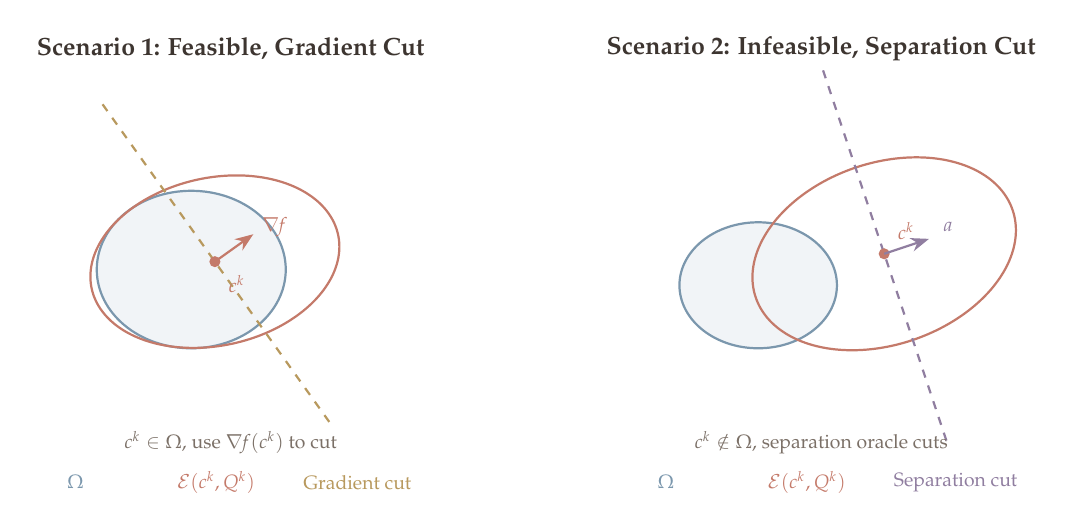
\begin{tikzpicture}[>=Stealth]

%%% Panel 1: Scenario 1 — Feasible, Gradient Cut
\begin{scope}[shift={(0,0)}]
  % Title
  \node[dkbrown, font=\small\bfseries] at (0,3.0) {Scenario 1: Feasible, Gradient Cut};

  % Omega (ellipse centered at (-0.5, 0.2), semi-axes 1.2, 1.0)
  \fill[bluefill, opacity=0.6] (-0.5, 0.2) ellipse (1.2 and 1.0);
  \draw[stblue, thick] (-0.5, 0.2) ellipse (1.2 and 1.0);

  % Ellipsoid E(c^k, Q^k): c1=(-0.2, 0.3)
  % L1=[[1.581,0],[0.190,1.079]]
  \draw[terracotta, thick]
    plot[domain=0:360, samples=200, smooth]
    ({1.581*cos(\x) + (-0.2)}, {0.190*cos(\x) + 1.079*sin(\x) + 0.3});

  % Gradient direction: (0.814, 0.581)
  % Hyperplane perpendicular: direction (-0.581, 0.814)
  % Cut line through c^k
  \draw[rwgold, thick, dashed]
    ({-0.2 - 2.5*(-0.581)}, {0.3 - 2.5*0.814})
    -- ({-0.2 + 2.5*(-0.581)}, {0.3 + 2.5*0.814});

  % Center
  \fill[terracotta] (-0.2, 0.3) circle (2pt);
  \node[terracotta, font=\scriptsize, below right] at (-0.15, 0.25) {$c^k$};

  % Gradient arrow
  \draw[->, terracotta, thick] (-0.2, 0.3) -- ({-0.2+0.6*0.814}, {0.3+0.6*0.581});
  \node[terracotta, font=\scriptsize] at ({-0.2+0.75*0.814+0.15}, {0.3+0.75*0.581}) {$\nabla\!f$};

  % Annotation
  \node[wmgray, font=\scriptsize] at (0, -2.0) {$c^k \in \Omega$, use $\nabla\!f(c^k)$ to cut};

  % Legend items
  \node[stblue, font=\scriptsize, right] at (-2.2, -2.5) {$\Omega$};
  \node[terracotta, font=\scriptsize, right] at (-0.8, -2.5) {$\mathcal{E}(c^k, Q^k)$};
  \node[rwgold, font=\scriptsize, right] at (0.8, -2.5) {Gradient cut};
\end{scope}

%%% Panel 2: Scenario 2 — Infeasible, Separation Cut
\begin{scope}[shift={(7.5,0)}]
  % Title
  \node[dkbrown, font=\small\bfseries] at (0,3.0) {Scenario 2: Infeasible, Separation Cut};

  % Omega (ellipse centered at (-0.8, 0), semi-axes 1.0, 0.8)
  \fill[bluefill, opacity=0.6] (-0.8, 0) ellipse (1.0 and 0.8);
  \draw[stblue, thick] (-0.8, 0) ellipse (1.0 and 0.8);

  % Ellipsoid E(c^k, Q^k): c2=(0.8, 0.4)
  % L2=[[1.673,0],[0.299,1.188]]
  \draw[terracotta, thick]
    plot[domain=0:360, samples=200, smooth]
    ({1.673*cos(\x) + 0.8}, {0.299*cos(\x) + 1.188*sin(\x) + 0.4});

  % Separation direction: (0.949, 0.316)
  % Hyperplane perpendicular: direction (-0.316, 0.949)
  % Cut line through c^k
  \draw[lavender, thick, dashed]
    ({0.8 - 2.5*(-0.316)}, {0.4 - 2.5*0.949})
    -- ({0.8 + 2.5*(-0.316)}, {0.4 + 2.5*0.949});

  % Center
  \fill[terracotta] (0.8, 0.4) circle (2pt);
  \node[terracotta, font=\scriptsize, above right] at (0.85, 0.45) {$c^k$};

  % Separation direction arrow
  \draw[->, lavender, thick] (0.8, 0.4) -- ({0.8+0.6*0.949}, {0.4+0.6*0.316});
  \node[lavender, font=\scriptsize] at ({0.8+0.75*0.949+0.1}, {0.4+0.75*0.316+0.1}) {$a$};

  % Annotation
  \node[wmgray, font=\scriptsize] at (0, -2.0) {$c^k \notin \Omega$, separation oracle cuts};

  % Legend items
  \node[stblue, font=\scriptsize, right] at (-2.2, -2.5) {$\Omega$};
  \node[terracotta, font=\scriptsize, right] at (-0.8, -2.5) {$\mathcal{E}(c^k, Q^k)$};
  \node[lavender, font=\scriptsize, right] at (0.8, -2.5) {Separation cut};
\end{scope}

\end{tikzpicture}
\end{document}
